\part{Decisões de projeto e implementação do trabalho}

\chapter[Decisões de engenharia a cerca do projeto]{Decisões de engenharia a cerca do projeto}

\section{Problemas atuais levantados nas Eclusas}

\subsection{Descrição dos problemas a serem tratados}

Tomando os requisitos levantados pela equipe que fica dentro das eclusas em conjunto com a equipe da sede, foram encontrados alguns problemas foram levantados para a melhor resolução do sistema. Entre os problemas mais críticos que podem ocorrer nas eclusas estão a falta de controle do nível de água no sistema de poços de adução e e esgotamento, a falta de semáforo na jusante e montante, a ausência de um software de supervisório \textit{SCADA} e o problemas de sincronização e controle nos servos motores da ponte.

Atualmente, os poços de adução e esgotamento não possuem um sistema de controle. Mesmo com sensores para monitorar os níveis de água e garantir que o processo de esvaziamento e enchimento das câmaras da eclusa ocorra de maneira controlada, todo o processo é feito de modo manual. A falta de um sistema instrumentalizado e eletronicamente controlado gera a operação ineficiente, podendo causar erros como o total enchimento dos poços, sendo problemático a retirada de água. 

O \textit{SCADA} é um sistema crítico para a supervisão e controle das operações de uma eclusa. A ausência de um software \textit{SCADA }pode resultar em monitoramento ineficiente, dificultando a monitoração dos processos em tempo real e reduzindo a capacidade de resposta a falhas e emergências. Além disso, há dificuldade na análise de dados, pois a coleta e análise de dados operacionais tornam-se limitadas, dificultando a identificação de padrões de desempenho e áreas que necessitam de melhorias. A falta de automação é outra consequência, já que a ausência de um software \textit{SCADA} impede a implementação de automação nos processos, o que poderia aumentar a eficiência e reduzir erros humanos.

Os semáforos são dispositivos essenciais para regular o tráfego de embarcações na entrada e saída das eclusas. A ausência desses semáforos pode causar confusão no tráfego, pois sem sinalização clara, as embarcações podem não saber quando é seguro entrar ou sair da eclusa, levando a possíveis colisões e congestionamentos. Isso resulta em atrasos operacionais, pois a falta de controle visual pode levar os operadores a se comunicarem manualmente com as embarcações para coordenar a passagem. Além disso, os riscos à segurança aumentam, já que a ausência de semáforos eleva a possibilidade de acidentes devido à falta de orientação clara.

Em suma, esses problemas destacados – falta de controle nos poços, problemas de sincronização nos servos motores da ponte, falta de um software de supervisório SCADA e falta de semáforo na jusante e montante – apresentam sérias consequências para a operação de eclusas, comprometendo a eficiência, a segurança e a manutenção das estruturas. A identificação e correção desses problemas são essenciais para garantir a operação segura e eficiente de uma eclusa.

\section{Análise dos problemas}

\subsection{Análise do tratamento da problemática}

Para analise dos problemas descritos, foram separados os problemas em 4 módulos, um módulo de inovação, sistemas auxiliares, supervisório e ponte. basicamente, o módulo de inovação irá resolver um item que antes não foi resolvido, que é a automação dos poços das eclusas. O sistema auxiliar será o controle dos semáforos que existem na montante e da jusante de uma eclusa. O supervisório será feito a partir de um software de código aberto com existência no mercado para a melhor observação do operador e a análise da ponte será feita através do estudo dos motores de passo.

\subsection{Módulo 01: Inovação}

Ao levantar os requisitos dos problemas das eclusas com a equipe de manutenção, um dos problemas foi o de controle dos níveis dos poços de adução e esgotamento. Um poço de adução é um poço onde se recebe a água bruta ou da jusante ou da montante e logo após é jogada para a câmara de eclusagem. Um poço de esgotamento é um poço onde a água da baixa da eclusagem é descarregada. 

Cada câmara contém 4 sensores redundantes de pressão que variam de 4 a 20mA e duas bombas, uma de 30cv na adução e outra de 45cv no esgotamento, como mostrado na figura \ref{fig:bombas}. a figura \ref{fig:sensor} mostra o sensor utilizado pelos poços. Segundo o datasheet do produto \cite{Gulton}, o Invólucro possui aço inoxidável AISI 304, possui Sinal de saída de 4 a 20mA, Resistência de carga de 0 a 1200 $\Omega$, 600 $\Omega$ para 24Vcc,  Alimentação de 12 a 36Vcc, sendo a alimentação típica de 24Vcc e Temperatura de operação: 0 a 60ºC.

\begin{figure}[h]
	\centering
	\label{fig:sensor}
		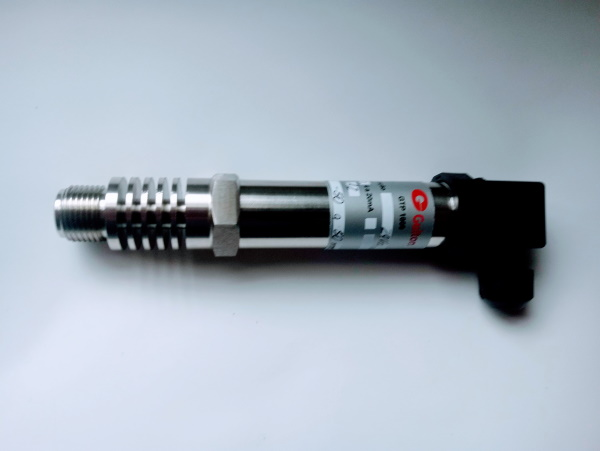
\includegraphics[keepaspectratio=true,scale=0.6]{figuras/GTP1000HT.jpg}
	\caption{Transmissor de pressão usado nos poços usado como sensor de nível}
\end{figure}

Para a automação dos poços, foi traçado uma lógica do processo de adução e esgotamento. A figura \ref{fig:diag_pocos} mostra o funcionamento básico. O sistema em si deve detectar o aumento do nível de água, verificar as fases da rede elétrica (para evitar o acionamento com fase invertida, fazendo com que a bomba coloque água no poço) e acionar o motor via inversor. Para o teste em paradigma será feito um modelo em escala menor, sendo seu passo a passo descrito no capítulo 04. 


\begin{figure}[h]
	\centering
	\label{fig:diag_pocos}
		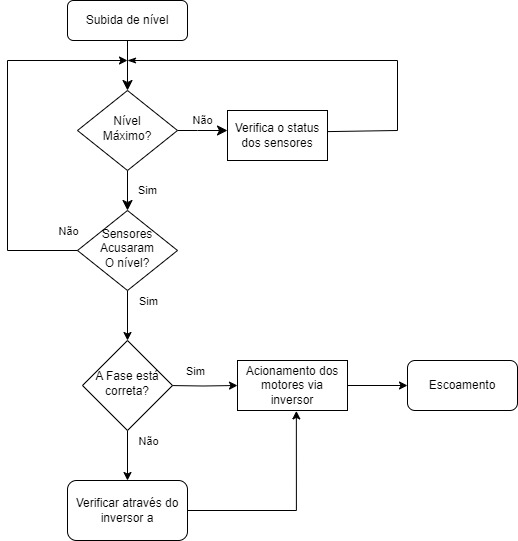
\includegraphics[keepaspectratio=true,scale=0.6]{figuras/pocos_new.jpg}
	\caption{Lógica básica do processo de adução e de esgotamento}
\end{figure}



\subsection{Módulo 02: Semáforos}


Os semáforos são componentes essenciais na operação de eclusas, garantindo a segurança e a eficiência do tráfego de embarcações. Eles regulam a entrada e a saída das embarcações, prevenindo colisões e otimizando o fluxo de tráfego.

Os semáforos em uma eclusa funcionam como sinais de trânsito que regulam a passagem de embarcações. Situados na jusante (parte inferior do rio) e montante (parte superior do rio) da eclusa, eles indicam aos navegantes quando é seguro entrar e sair das câmaras. Esse controle é fundamental para coordenar o trânsito de embarcações, especialmente em vias navegáveis movimentadas, onde a segurança e a eficiência são prioridades.

Para garantir a operação segura e eficiente das eclusas, é crucial implementar e manter adequadamente os sistemas de semáforos. Para o projeto se usará um microcontrolador ligado aos semáforos e ao sistema de supervisório. 

A integração dos semáforos aos sistema de supervisório deve permitir que suas operações sejam coordenadas automaticamente com outros processos, como o enchimento e esvaziamento das câmaras. Essa integração melhora a eficiência e reduz a necessidade de intervenção manual.


\subsection{Módulo 03: O Supervisório}

A operação eficiente e segura de uma eclusa depende de um controle rigoroso e da supervisão contínua de vários parâmetros operacionais. Um sistema supervisório \textit{SCADA} é importante para o monitoramento e o controle dos parâmetros em tempo real.

\begin{figure}[h]
	\centering
	\label{fig:diag_pocos}
		
\includegraphics[keepaspectratio=true,scale=0.6]{figuras/scadabr_logo.png}
	\caption{SCADABR logo}
\end{figure}

Os sistemas supervisórios \textit{SCADA} são projetados para coletar dados em tempo real, processá-los e exibir informações críticas para os operadores. Em uma eclusa, esses sistemas desempenham várias funções vitais, das quais estão o Monitoramento em tempo real, o controle e a automação dos processos, o registro de dados em um banco de dados para análise posterior, alarmes e notificações e a integração de vários sistemas.

O \textit{SCADA} permite a visualização e o monitoramento em tempo real dos níveis de água, status de portas, bombas, válvulas e outros componentes críticos da eclusa. Isso possibilita uma resposta imediata a qualquer anomalia, minimizando o risco de falhas operacionais. Os sistemas \textit{SCADA} facilitam o controle automatizado das operações da eclusa, como o enchimento e esvaziamento das câmaras, abertura e fechamento de portas e operação de sistemas auxiliares. A automação reduz a dependência de intervenção manual, aumentando a eficiência e a precisão das operações.O \textit{SCADA} armazena dados históricos que são essenciais para análises de desempenho, identificação de tendências e planejamento de manutenção preventiva. Isso ajuda na tomada de decisões informadas e na melhoria contínua das operações.O sistema pode ser configurado para gerar alarmes e notificações em caso de condições anômalas, como níveis de água fora dos limites, falhas em equipamentos ou situações de emergência. Isso permite uma resposta rápida e eficaz para mitigar riscos.

Um sistema \textit{SCADA} pode ser integrado com outros sistemas de controle e gestão, proporcionando uma visão holística das operações e facilitando a coordenação entre diferentes componentes e processos da eclusa. De acordo com \cite{scadabr_manual} O SCADABR é uma solução de código aberto, o que o torna uma opção economicamente viável, especialmente para projetos com orçamento limitado. A ausência de licenças de software caras reduz significativamente os custos iniciais e de manutenção.Como um projeto de código aberto, o SCADABR possui uma comunidade ativa de desenvolvedores e usuários que contribuem com melhorias contínuas, documentação e suporte. Esse aspecto comunitário garante que o sistema evolua e se mantenha atualizado com as melhores práticas do setor.


\begin{figure}[h]
	\centering
	\label{fig:diag_pocos}
		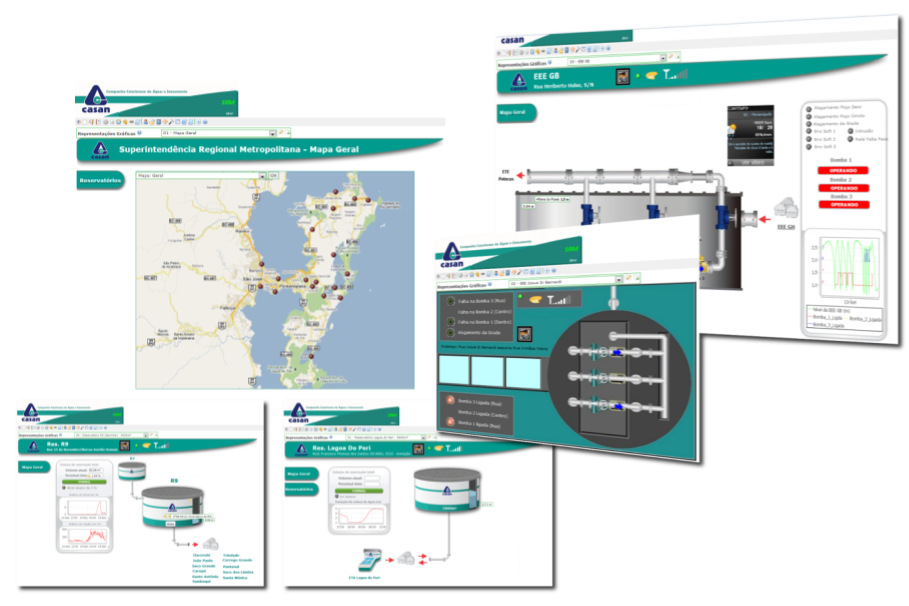
\includegraphics[keepaspectratio=true,scale=0.3]{figuras/dashboard_scadabr.png}
	\caption{Vários dashboards produzidos pelo SCADABR (Fonte: Companhia de Saneamento Catarinense)}
\end{figure}


\subsection{Modulo 04: Ponte}


A ponte de uma eclusa desempenha um papel vital na integração de transporte terrestre e fluvial, permitindo a passagem de veículos e pedestres sobre a estrutura enquanto regula a entrada e saída das embarcações. A operação eficaz desta ponte depende fortemente dos servos motores, que controlam seu movimento. Este capítulo examina a função da ponte, a importância dos servos motores, os problemas de sincronização e as melhores práticas para a sua manutenção e operação.

As pontes em eclusas são projetadas para se mover, permitindo a passagem de embarcações de diferentes alturas e garantindo o fluxo contínuo de tráfego terrestre. Existem diferentes tipos de pontes móveis, como pontes levadiças, basculantes e giratórias, cada uma projetada para atender às necessidades específicas do local.

A função principal dessas pontes inclui: Permitir a Navegação, Ao se levantar ou girar, a ponte permite que embarcações maiores passem através da eclusa, ajustando-se às variações de nível da água.
Garantir a Conectividade Terrestre, Quando abaixada ou em posição fechada, a ponte proporciona um caminho seguro para veículos e pedestres, mantendo a conectividade entre as duas margens do curso d'água.
Os servos motores são dispositivos críticos que controlam o movimento das pontes móveis. Eles são responsáveis por garantir que a ponte opere suavemente, de forma coordenada e segura. Os servos motores são fundamentais por várias razões. Eles fornecem um controle preciso sobre a velocidade e a posição da ponte, permitindo operações seguras e eficientes.Servos motores garantem que todos os componentes móveis da ponte operem em perfeita harmonia, evitando desalinhamentos que possam causar danos à estrutura. São projetados para suportar cargas pesadas e operar em condições ambientais adversas, garantindo a longevidade da ponte. Facilitam a automação do movimento da ponte, reduzindo a necessidade de intervenção manual e aumentando a eficiência operacional.

Para o controle dos motores será feito um estudo sobre a ponte e como uma lógica de motores pode melhorar e otimizar o processo como um todo.